\documentclass[12pt,a4paper,twoside]{article}
\usepackage[utf8]{inputenc}
\usepackage{amsmath}
\usepackage{lmodern}
\usepackage{textcomp}
\usepackage{amsfonts}
\usepackage{amssymb}
\usepackage{graphicx}
\usepackage[left=2cm,right=2cm,top=2cm,bottom=2cm]{geometry}
\author{Eduardo Castillo Bastida}
% used in maketitle                                                             
\title{\textbf{Movimiento de la Tierra y la Luna Alrededor del Sol}}
\begin{document}
\maketitle
El presente estudio del movimiento de la tierra y la luna alrededor del sol, se centra en considerar el movimiento descrito por una trayectoria circular de la tierra respecto al sol, mientras la luna describe el mismo movimiento alrededor de la tierra. Para tal fin se considera a la tierra y la luna discribiendo una circunferencia al rededor del sol y la luna alrededor de la tierra, con un radio medio de R=1496000000 km, y r=149600000 km, respectivamente, como muestra la gráfica 1. 
\begin{figure}[htbp]
\centering
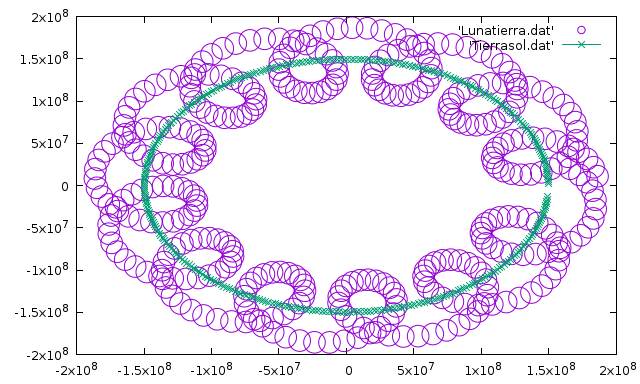
\includegraphics[width=12cm]{Sistema.png}
\caption{Trayectoria de la tierra y la luna alrededor del sol.}\label{fig:figura1}
\end{figure}
La trayectoria de al tierra alrededor del sol, corresponde una una circunferencia descrita por la ecuación en coordenadas polares, dada como:
\begin{eqnarray}
R=1496000000
\end{eqnarray}
En termino de coordenadas cartesianas, esta trayectoria puede ser expresada por las ecuaciones:
\begin{eqnarray}
x_{t}=Rcos(\theta)\\
y_{t}=Rsin(\theta)
\end{eqnarray}
Donde $\theta$ corresponde al ángulo barrido por el radio de la tierra al sol.
La trayectoria de la luna respecto a la tierra, mientras la tierra se mueve, es el resultado de un movimiento relativo respecto al sol descrito por las ecuaciones:
\begin{eqnarray}
x_{_{l}}=Rcos(\theta)+rcos(\alpha)\\
y_{l}=Rsin(\theta)+rsin(\alpha)
\end{eqnarray}
Donde $\alpha$ corresponde al ángulo barrido por el radio de la luna a la tierra.
\section{Aplicación Fortran para el cálculo de la trayectoria de la la tierra alrededor del sol}
El código de la aplicación fortran para determinar la trayectoria en coordenadas cartesianas de la tierra y la luna alrededor del sol, corresponde a:
\begin{verbatim}
function solx(asol) result (x)
	double precision, intent(in) :: asol
	double precision 	     :: x
        double precision, parameter :: rsol = 1.496d8
	 x = rsol * dcos(asol)
end function solx
function soly(asol) result (y)
	double precision, intent(in) :: asol
	double precision 	     :: y
	double precision, parameter :: rsol = 1.496d8
	 y = rsol * dsin(asol)
end function soly

subroutine moon(rsol, rluna, posx, posy, alun, asol)
   double precision, intent (in) :: rsol, alun, asol
   double precision, intent (out) :: posx, posy
   double precision :: rluna
   rluna = rsol / 4.0d0
   posx = (rsol * dcos(asol)) +(rluna * dcos(alun))
   posy = (rsol * dsin(asol)) +(rluna * dsin(alun))

end subroutine moon


program luna
	implicit none
	integer :: i
	double precision :: g, dia, rsol, rluna, posx, posy, alun
	double precision :: rad, velluna, velsol, solx, soly, asol
	double precision, parameter :: pi=3.1416d0, month = 27.3217d0, year = 365.26d0
	double precision, dimension(360) :: totx,toty
	double precision, dimension(360) :: x, y
  rsol = 1.496d8
  rad = pi / 180.0d0
  dia = 365.26d0/(360.0d0*rad) !para saber cuantos dias pasan por radian
  velluna = 2.0d0 * (pi / month) !Es lo que recorre diariamente la luna en radianes
  velsol = 2.0d0 * (pi / year)

open (1, file = 'LunaVtierra.dat', status = 'unknown')
open (2, file = 'TierrAsol.dat', status = 'unknown')
 do i=1, 360, 1
 g = dble(i)
 asol = g * velsol
 alun = g * velluna  !para saber la posicion actual en radianes
 x(i) = solx(asol)
 y(i) = soly(asol) !Las posiciones dadas por la funcion, para la posicion de la tierra respecto al sol
 call moon(rsol, rluna, posx, posy, alun, asol)  !para calcular la posicion de la luna respecto a la tierra y el sol
 totx(i) = posx
 toty(i) = posy
 write (1,*) totx(i), toty(i)
 write (1,*) ' '
 write (2,*) x(i), y(i)
 write (2,*) ' '

 end do
 close (1)
 close (2)
end program luna

\end{verbatim}
\end{document}
